    \documentclass[conference]{IEEEtran}
    \usepackage{cite}
    \usepackage{amsmath,amssymb,amsfonts}
    \usepackage{algorithmic}
    \usepackage{graphicx}
    \usepackage{textcomp}
    \usepackage{xcolor}
    \usepackage{hyperref}

\begin{document}

\title{2D Planar Hopping Robot Quadratic MPC}

\author{\IEEEauthorblockN{Misha Lvovsky}}

\maketitle

\begin{abstract}
    The goal of this project is to implement an MPC (Model Predictive Controller) for a single legged hopping robot.
    The MPC will be formulated as a Quadratic Program (QP) and will be solved using an off-the-shelf solver in python.
    The setup of the robot is a square body with a single 1p leg and a reaction wheel that allows it to apply forces perpendicular to its leg.
\end{abstract}

\section{Introduction}
\label{sec:introduction}


\subsection{Historical Background}

The control of simple hopping robots has been studied as early as 1984 when Marc Raibert built and subsequently studied the single legged Raibert Hopper \cite{raibert_experiments_1984}.
The control of such robots is a reduced version of the control of legged robots with more than one leg, making it a popular field of study and testing grounds for new algorithms for legged robots.

MPCs have emerged as one of the best ways to control highly dynamic systems such as legged robots.
MPCs started in other slower dynamic systems before they were used in legged robots.
In fact, MPCs have been studied since the 60s when they were developed for use in the control of chemical processes such as this work by Chestnut et al. \cite{chestnut_predictive-control_1961}.
The use of MPCs for legged robots however is a more recent development that began as the processing power necessary to solve for the control inputs of a robot on-board became available, as well as the hardware necessary to make legged robots feasible started to develop.
The first use of MPC to control legged robot motions online was done by Christine Azevedo in 2002 where she used an MPC to solve for control of a bipedal robot \cite{azevedo_line_2002}.

Since then this the topic has been studied in much more detail resulting in MPCs which are deployed on much faster and more dynamic robots.

\subsection{Recent Work}

More recently the use of MPCs has extended to the onboard online optimization of legged robot control sequences such as the one studied by Erez et al. \cite{erez_integrated_2013}.
These MPCs have ranged from highly nonlinear MPCs that simultaneously optimize the landing locations, times, and reaction forces, to simpler methods which eschew the more complex aspects of the problem often converting it to a convex optimization problem which can be solved at a high frequency and thus provide highly relevant trajectories that are updated to the robot's current state.

An additional direction of recent development has been in the use of various techniques to leverage prior data to speed up or stabilize the optimization process.
One such example is the use of learned function approximators investigated by Melon et al. to give a warm starting guess to speed up the optimization convergence \cite{melon_receding-horizon_2021}.
Another example is the use of heuristics to make the non-convex problem closer to a convex one preventing convergence in local minima and thus making the optimization far more robust such as the method investigated by Bledt and Kim \cite{bledt_extracting_2020}.

A second direction of recent development is in the use of contact implicit solvers to merge the optimization of contact and control at the same time, allowing the discovery of more optimal control inputs and position trajectories.
An example of an investigation in this direction is the one conducted by Le Cleac and Howell et al. \cite{cleach_fast_2023} which uses complementarity to find contact implicit trajectories.
Another is one led by Toussaint et al. \cite{toussaint_sequence--constraints_2022} which uses a sequence of constraints to force the desired behavior.

\section{Background}
\label{sec:background}

MPC problems are optimization problems of the standard form that optimize a cost function \(J(x)\) and given constraint functions \(g(x)\) and \(h(x)\) find the \(x\) that minimizes \(J(x)\) subject to the constraint that \(g(x)\leq0\) and \(g(x)=0\).

\begin{align*}
    \quad & x                &                                           & \text{Optimization Variable} \\
          & J                &                                           & \text{Cost Function}         \\
          & g \text{ and } h &                                           & \text{Constraint Functions}  \\
          &                  & x^* = \underset{x}{\text{argmin}} \; J(x)                                \\
          & \text{S.T.}      &                                                                          \\
          &                  & g(x) \leq 0                                                              \\
          &                  & h(x) = 0
\end{align*}

When this form is used for MPC the cost function is formulated such that some portion of \(x\) can be used to compute the optimal control input, and the constraints keep that control feasible.
There exist a variety of ways to formulate such a cost function.

Naunert et al. \cite{neunert_whole-body_2018} specify a collocation constraint using realistic nonlinear robot dynamics and a cost function of an arbitrary form \(L(x, u, t)\) integrated over the trajectory as well as a cost on the final position \(h(x_f)\).
Posa et al. \cite{posa_direct_2014} and Le Cleac and Howell et al. \cite{cleach_fast_2023} take a similar approach but use complementarity to implicitly solve for contacts and reaction forces simultaneously.
The complementarity comes from the requirement that either contact distances are zero or contact forces are zero.

The works that this project is adapting to the planar 2D monopod case are the work of of Kim et al. \cite{kim_highly_2019} and Di Carlo et al. \cite{di_carlo_dynamic_2018} on optimizing reaction forces for the control of fast legged robots.
These works further distill the problem down from the other formulations mentioned to reduce all the way to a QP optimization problem subject to linear constraints that can be solved extremely quickly on-board a small mobile robot.
By using an abstraction which captures enough of the robot's dynamics to generate useful control trajectories in a form that is easy for optimization engines to solve, these formulations are able to update extremely quickly and thus reject errors more effectively.

\section{Methodology}
\label{sec:methodology}

To begin formulating the optimization problem we will stack the optimization variables into vectors

\[x_t = \begin{bmatrix} \theta_t\: \vec{r}^T_t \dot{\theta}_t\: \dot{\vec{r}}^T_t \end{bmatrix}^T\]
\[u_t = \begin{bmatrix} f_x\: f_y\end{bmatrix}^T\]

where \(\vec{r}_t\) is the position of the robot's body at time \(t\), \(\theta_t\) is the angle, and \(f_x\) and \(f_y\) are the reaction forces from the ground.

\begin{figure}[h!]
    \centering
    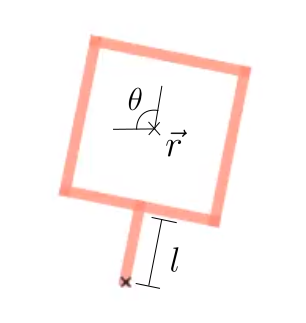
\includegraphics[width=0.4\textwidth]{robot.png}
    \caption{
        This is the 2D planar biped being controlled.
        This figure shows the \(\theta\), \(\vec{r}\), and \(l\) state elements on the system.
    }
    \label{fig:robot}
\end{figure}


Now we can begin to make simplifications to the dynamics of the robot in order to get it into the right form for QP.

\[\frac{d}{dt}x=\begin{bmatrix} \mathbf{I} & \mathbf{I}dt \\ \mathbf{0} & \mathbf{I} \end{bmatrix} x + \begin{bmatrix} \mathbf{0} & \mathbf{0} \\ \mathbf{0} & \mathbf{M} \end{bmatrix} \begin{bmatrix} \mathbf{0} \\ J_t \end{bmatrix} u = Ax + Bu \]

Where \(\mathbf{M}\) is the mass matrix and \(A\) and \(B\) are calculated from \(\mathbf{M}\) and \(dt\).\
This simplification ignores the coriolis effects, assuming that in the absence of control force there will be no acceleration whatsoever.
This is not correct in our case since our system has coriolis forces linking the rotation of the body to the length of the leg.
However, this model is a good approximation when the speed is relatively low and the leg is short.

The friction constraint enforces that \(\|f_x\| \leq \mu f_y\).
The contact constraint  enforces that \(f_y > \epsilon\).
Where \(\epsilon\) is some small value to ensure that the foot remains planted on the ground.
Expressing this as a matrix for the QP solver gives the following.
\[
    \begin{bmatrix}
        -1.0 & -\mu \\
        1.0  & -\mu \\
        0    & -1.0 \\
    \end{bmatrix} u \leq \begin{bmatrix}
        0.0       \\
        0.0       \\
        -\epsilon \\
    \end{bmatrix}
\]

Now to simplify the QP we will further coalesce these representations into one which is easily representable by a few matrix products.
First we will reformulate the dynamics in terms of two matrices \(\mathbf{A}_\text{qp}\) and \(\mathbf{B}_\text{qp}\) which have the form:

\[\mathbf{A}_{qp} = \begin{bmatrix} \mathbf{I}\: A^T\: A^{2T} \cdots A^{nT}\: \end{bmatrix}\]
\[
    \mathbf{B}_{qp} = \begin{bmatrix}
        \mathbf{0} & \mathbf{0} & \mathbf{0} & \cdots & \mathbf{0} \\
        b_0        & \mathbf{0} & \mathbf{0} & \cdots & \mathbf{0} \\
        Ab_0       & b_1        & 0          & \cdots & 0          \\
        A^2b_0     & Ab_1       & b_2        & \cdots & \mathbf{0} \\
        \vdots     & \vdots     & \vdots     & \ddots & \vdots     \\
        A^nb_0     & A^{n-1}b_1 & A^{n-2}b_2 & \hdots & b_n        \\
    \end{bmatrix}
\]
\[\mathbf{X} = \left[\begin{smallmatrix} \mathbf{x}_0^T\: \mathbf{x}_1^T \cdots\: \mathbf{x}_n^T\end{smallmatrix} \right]^T\]

Given these matrices we can now reformulate the dynamics as follows.
\[\mathbf{X} = \mathbf{A}_\text{qp}\mathbf{x}_0 + \mathbf{B}U\]

Now that we have simplified the dynamics we can forumlate cost function.
\[\|\mathbf{A}_\text{qp}\mathbf{x}_0+\mathbf{B}_\text{qp}\mathbf{U}-\mathbf{x}_\text{ref} \|_\mathbf{L} + \|U\|_\mathbf{K}\]

Where \(\|P\|_Q\) represents \(Q^TPQ\).
Rearranging this into standard QP form gives:

\begin{align*}\min\limits_\mathbf{U}\frac12\mathbf{U}^T\mathbf{H}\mathbf{U} + \mathbf{U}^Tg
     & \min\limits_\mathbf{U} & \frac12\mathbf{U}^T\mathbf{H}\mathbf{U} + \mathbf{U}^Tg \\
     & \text{s.  t.}          & \mathbf{CU} \leq \bar{c}
\end{align*}

Where \(\mathbf{C}\) is defined as the constraint matrix defined earlier expanded to all time steps
\[\mathbf{C} = \begin{bmatrix}
        -1.0 & -\mu \\
        1.0  & -\mu \\
        0    & -1.0 \\
    \end{bmatrix}^{\otimes n} \]
\[\bar{c} =  \begin{bmatrix}
        0.0       \\
        0.0       \\
        -\epsilon \\
    \end{bmatrix}^{\otimes n}\]

Optimizing this quadratic objective and linear constraint results in a set of control inputs that make the robot track the reference trajectory.

\section{Results}
\label{sec:results}

The first set of results is from a simulated experiment of running the robot attempting to make a few different size hops one after another.
The results of this experiment are in figure~\ref{fig:fig2}.
From the results of this plot we can see that based on the convergence of the x position to the target we have a successful controller.
The x position command changes and then we can see that the robot arrives at that position after one bounce.

\begin{figure}[h!]
    \centering
    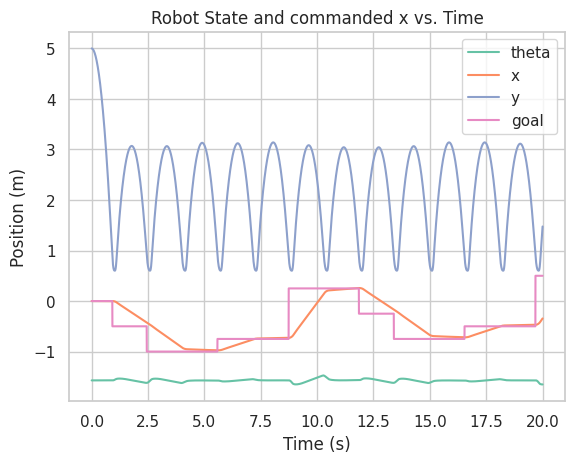
\includegraphics[width=0.4\textwidth]{fig2.png}
    \caption{
        The x axis of this plot corresponds to the time of the state that is plotted on the y axis.
        The y axis is the value of the variable in question, which is different for each colored line.
        The blue line shows the y height of the robot, the orange shows the x position, green shows the theta at that time, and red shows the target x pos for the robot to end up in.
    }
    \label{fig:fig2}
\end{figure}

An additional metric by which the performance of this controller can be measured is by the success with which the controller adhered to the commanded air time.
In figure~\ref{fig:fig2} I used an air time of 1.5 seconds for all data since this seems to be the ideal point for the studied MPC.
Figure~\ref{fig:fig3} shows the distribution of the achieved air times for a given commanded air time.
The reason for the inaccuracy to the trajectory at the higher end is due to the simplification made to not use effects dependent on velocity.
Once a large enough velocity is commanded these effects become relevant and accuracy is lost.

\begin{figure}[h!]
    \centering
    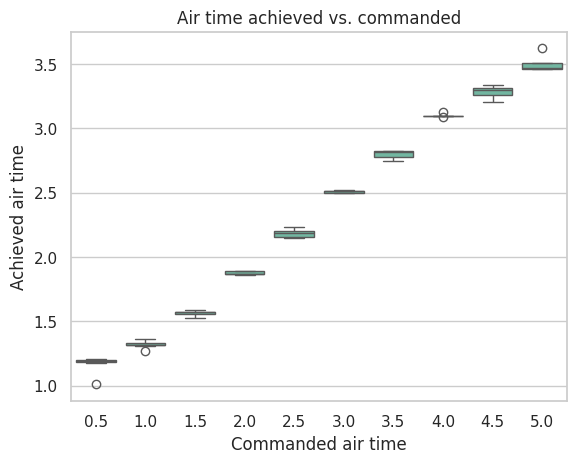
\includegraphics[width=0.4\textwidth]{fig3.png}
    \caption{
        The x axis of this plot corresponds to the commanded air time.
        Each column contains a box plot but they are very dense because the variation in height is very small.
        The y axis is the air time that the robot actually achieved in simulation.
    }
    \label{fig:fig3}
\end{figure}

\section{Conclusion}
\label{sec:conclusion}

This project successfuly adapter the trajectory optimization algorithm to the 2D monopod system and controlled it to follow some reference trajectories.
This success despite the limitations of the simplicity of the model and the sub-optimality of the trajectory generator highlight the positive properties of MPC control, namely that because of the predictive control it is reasonably robust to dynamics immprecision.

The challenges enountered were primarily in generating feasible reference trajectories that lead to feasible contact sequences.

An interesting area of future investigation would be improvement upon the achieved air times either by switching to some variety of nonlinear model or improving the formulation of the QP model.
Another interesting area of future investigation would be to try various more advanced trajectory generators than the simple heuristic one used for this investigation.

In conclusion, this project was great for getting more familiar with the MPC algorithm.
Though I was aware of this algorithm prior to doing this assignment I still found myself referncing various papers often.
I learned a lot throught the process of implementing this final project and am happy with the reasonably successful result.

\bibliographystyle{IEEEtran}
\bibliography{references}

\end{document}
